\documentclass[compress]{beamer}
\usepackage{ifthen,verbatim}

\title{Misalignment and Track-based Alignment}
\author{Jim Pivarski, Alexei Safonov}
\institute{Texas A\&M University}
\date{17 January, 2008}

\newcommand{\isnote}{}
\xdefinecolor{lightyellow}{rgb}{1.,1.,0.25}
\xdefinecolor{darkblue}{rgb}{0.1,0.1,0.7}

%% Uncomment this to get annotations
%% \def\notes{\addtocounter{page}{-1}
%%            \renewcommand{\isnote}{*}
%% 	   \beamertemplateshadingbackground{lightyellow}{white}
%%            \begin{frame}
%%            \frametitle{Notes for the previous page (page \insertpagenumber)}
%%            \itemize}
%% \def\endnotes{\enditemize
%% 	      \end{frame}
%%               \beamertemplateshadingbackground{white}{white}
%%               \renewcommand{\isnote}{}}

%% Uncomment this to not get annotations
\def\notes{\comment}
\def\endnotes{\endcomment}

\setbeamertemplate{navigation symbols}{}
\setbeamertemplate{headline}{\includegraphics[height=1 cm]{../cmslogo} \hspace{0.1 cm} \includegraphics[height=1 cm]{../tamulogo} \hfill
\begin{minipage}{5.5 cm}
\vspace{-0.75 cm} \small
\begin{center}
\ifthenelse{\equal{\insertpagenumber}{1}}{}{\textcolor{blue}{\insertsection}}
\end{center}
\end{minipage} \hfill
\begin{minipage}{4.5 cm}
\vspace{-0.75 cm} \small
\begin{flushright}
\ifthenelse{\equal{\insertpagenumber}{1}}{}{Jim Pivarski \hspace{0.5 cm} \insertpagenumber\isnote/\pageref{numpages}}
\end{flushright}
\end{minipage}\mbox{\hspace{0.2 cm}}}

\begin{document}
\frame{\titlepage}

%% \begin{notes}
%% \item This is the annotated version of my talk.
%% \item If you want the version that I am presenting, download the one
%% labeled ``slides'' on Indico (or just ignore these yellow pages).
%% \item The annotated version is provided for extra detail and a written
%% record of comments that I intend to make orally.
%% \item Yellow notes refer to the content on the {\it previous} page.
%% \item All other slides are identical for the two versions.
%% \end{notes}

\begin{frame}
\begin{itemize}\setlength{\itemsep}{0.75 cm}
\item Scaled 10~pb$^{-1}$ to 100~pb$^{-1}$, updated all plots
\item Results did not show anticipated improvement: began investigation
\item Lead to improvements in the alignment procedure, but that's for a different meeting
\item The new plots
\end{itemize}
\end{frame}

\begin{frame}
\frametitle{Side-by-side comparison (alignment position error)}

9 passes $\times$ 5 iterations, only 2 stations aligned per pass

\vspace{0.2 cm}
``Chamber $x$ position RMS'' is $\sqrt{\overline{(x_{\mbox{\scriptsize true}} - x_{\mbox{\scriptsize aligned}})^2}}$, includes offsets

\vspace{-0.2 cm}
\begin{columns}
\column{0.5\linewidth}
\begin{center} \textcolor{darkblue}{10~pb$^{-1}$ alignment} \end{center}

\vspace{-0.25 cm}
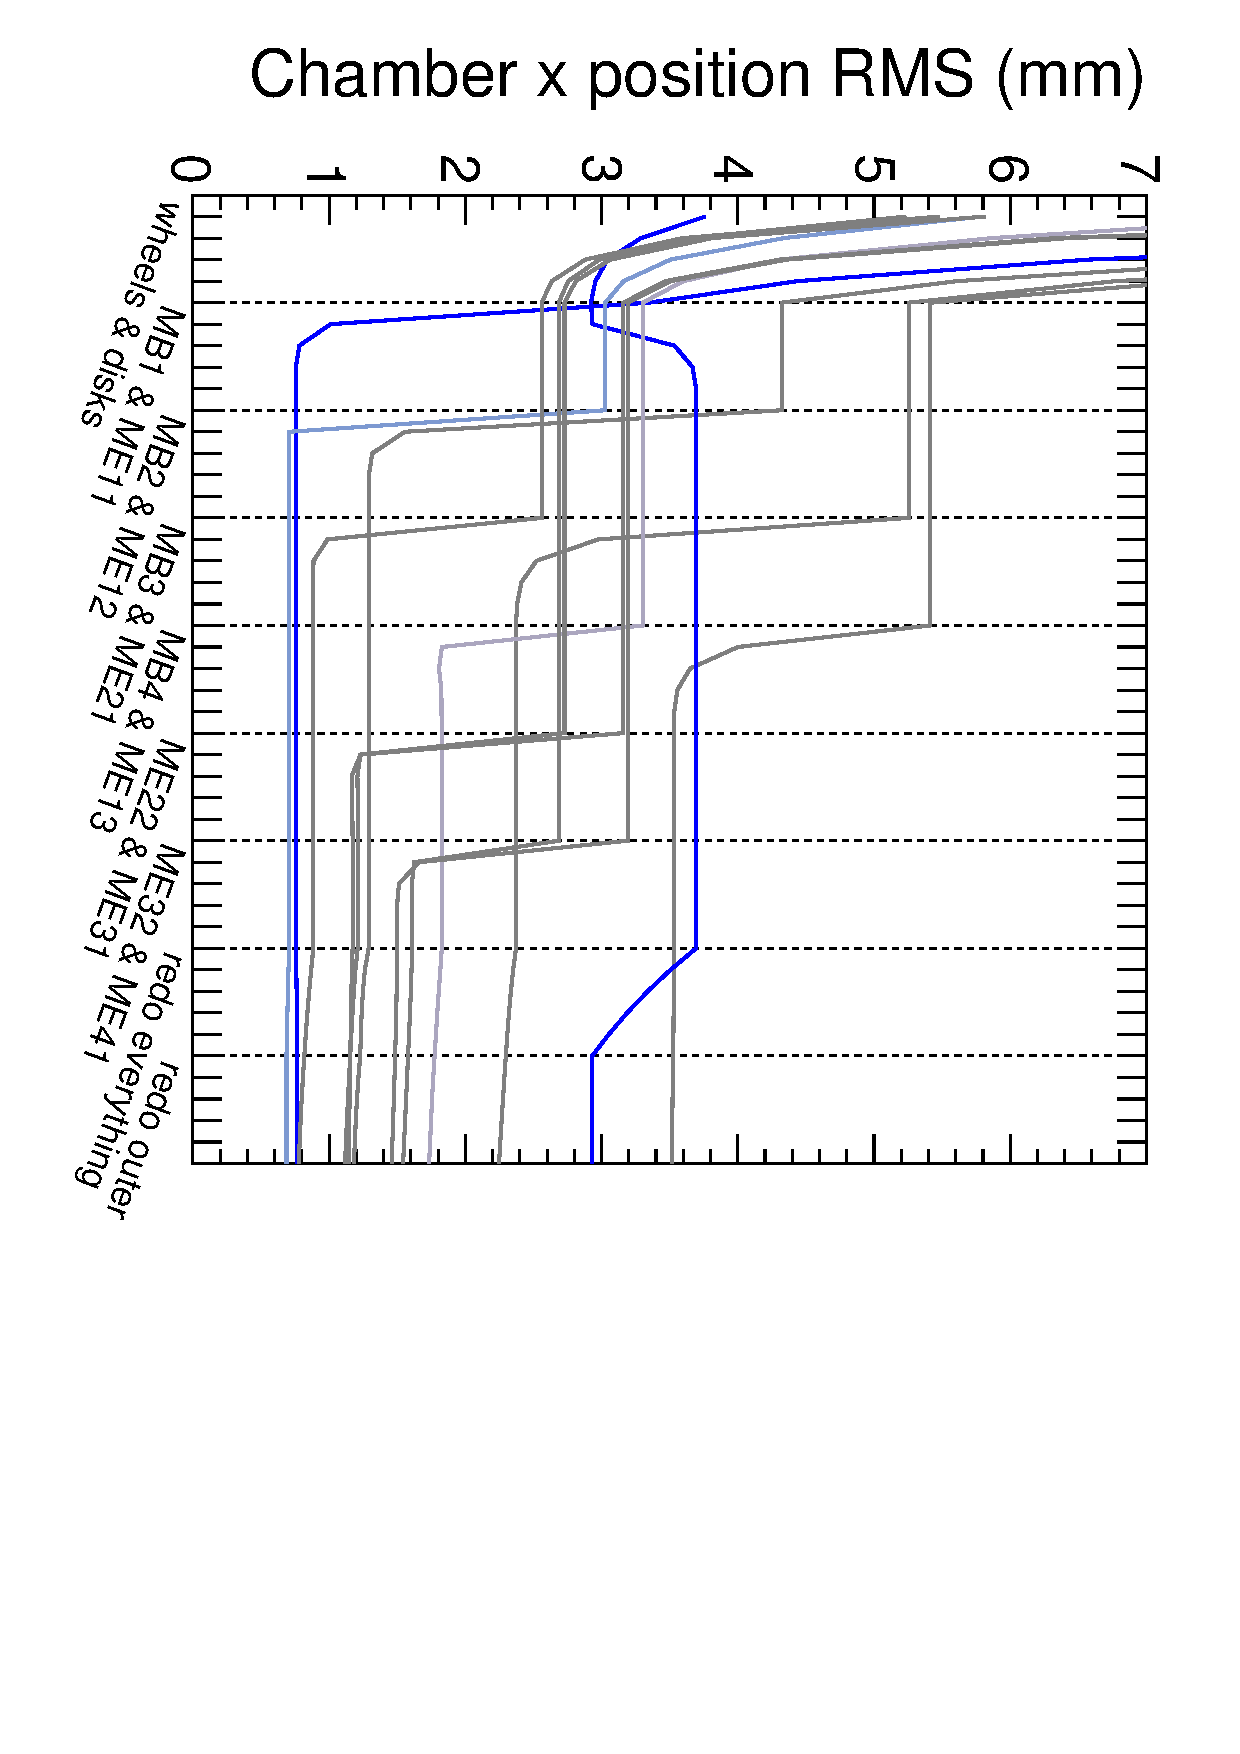
\includegraphics[height=\linewidth, angle=90]{convergence-10.pdf}

\column{0.5\linewidth}
\begin{center} \textcolor{darkblue}{100~pb$^{-1}$ alignment} \end{center}

\vspace{-0.25 cm}
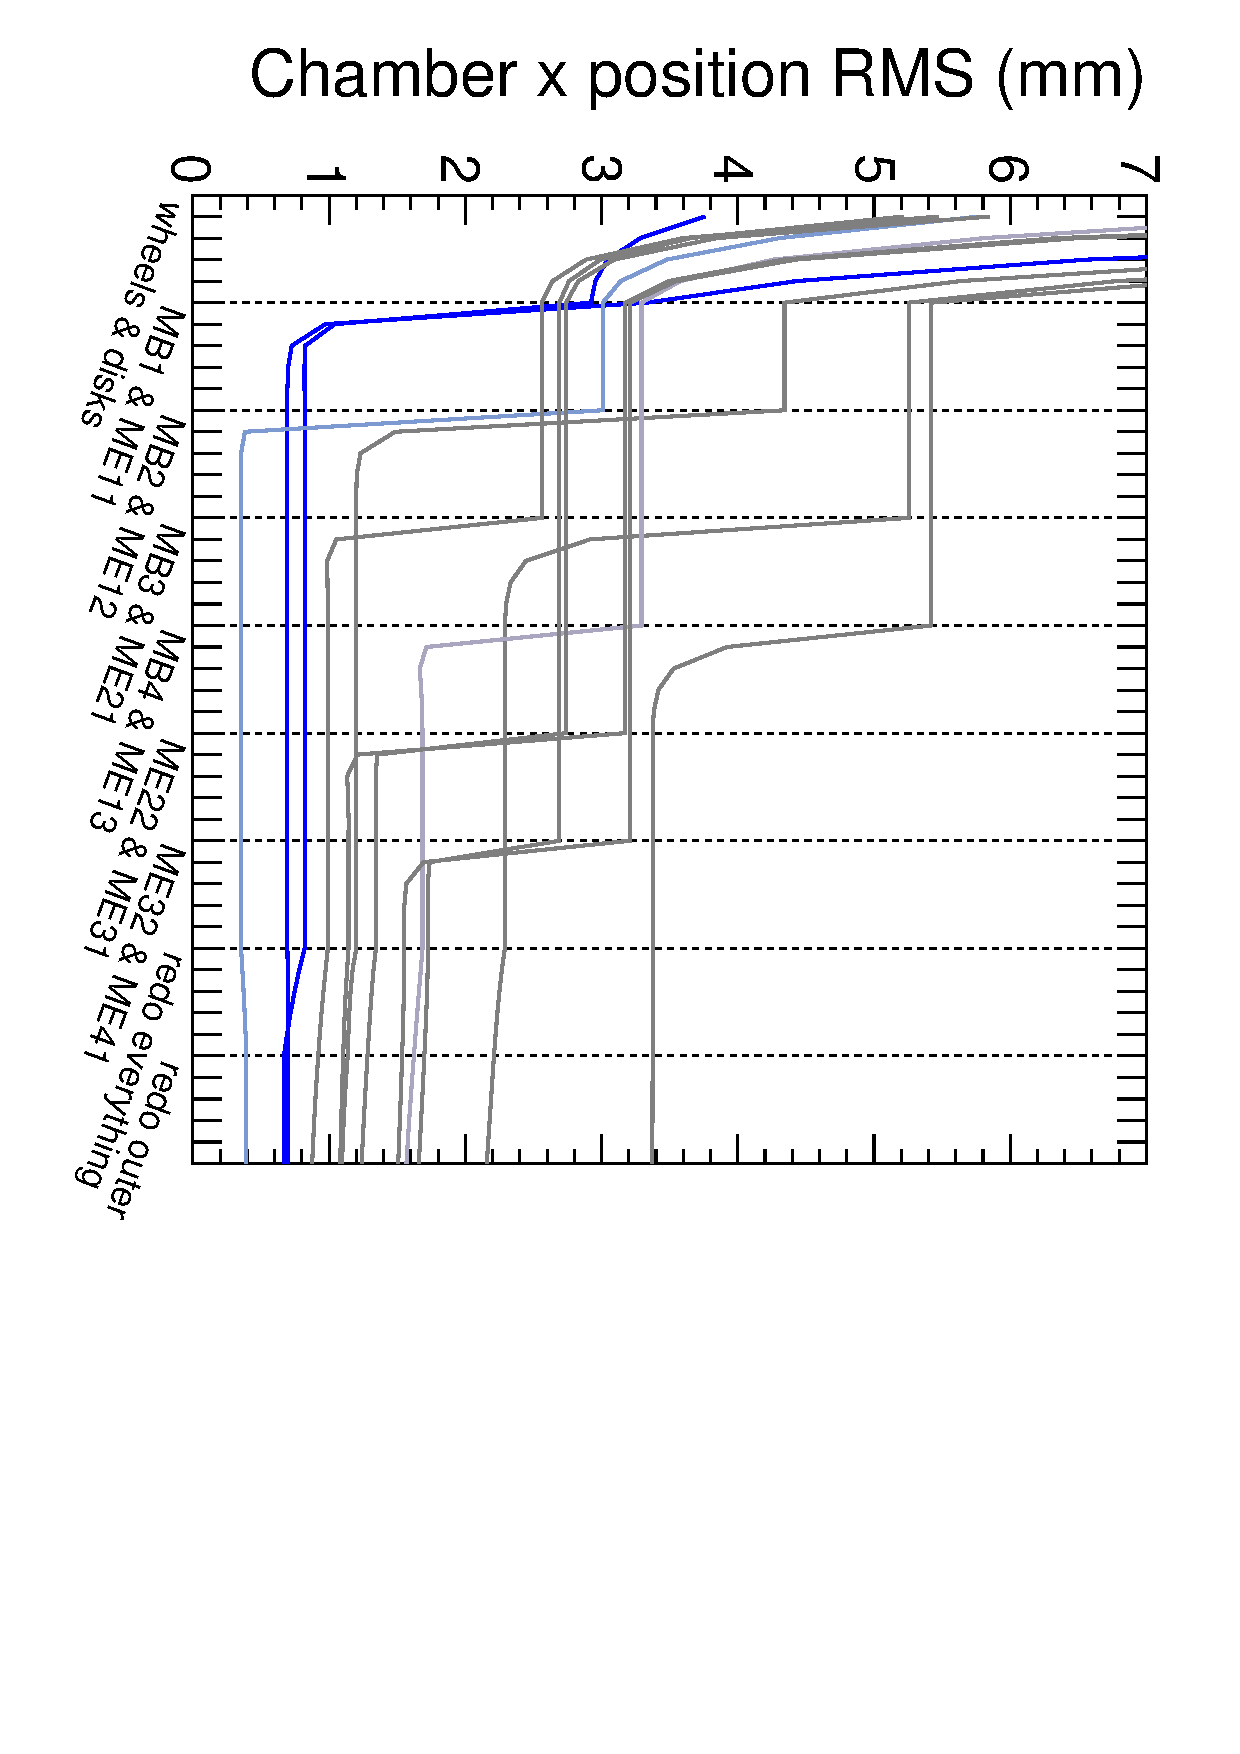
\includegraphics[height=\linewidth, angle=90]{convergence-100.pdf}
\end{columns}
\end{frame}

\begin{frame}
\frametitle{Overlaid comparison (alignment position error)}

\begin{center} \textcolor{red}{red: 10~pb$^{-1}$} \hspace{0.5 cm} \textcolor{blue}{blue: 100~pb$^{-1}$}

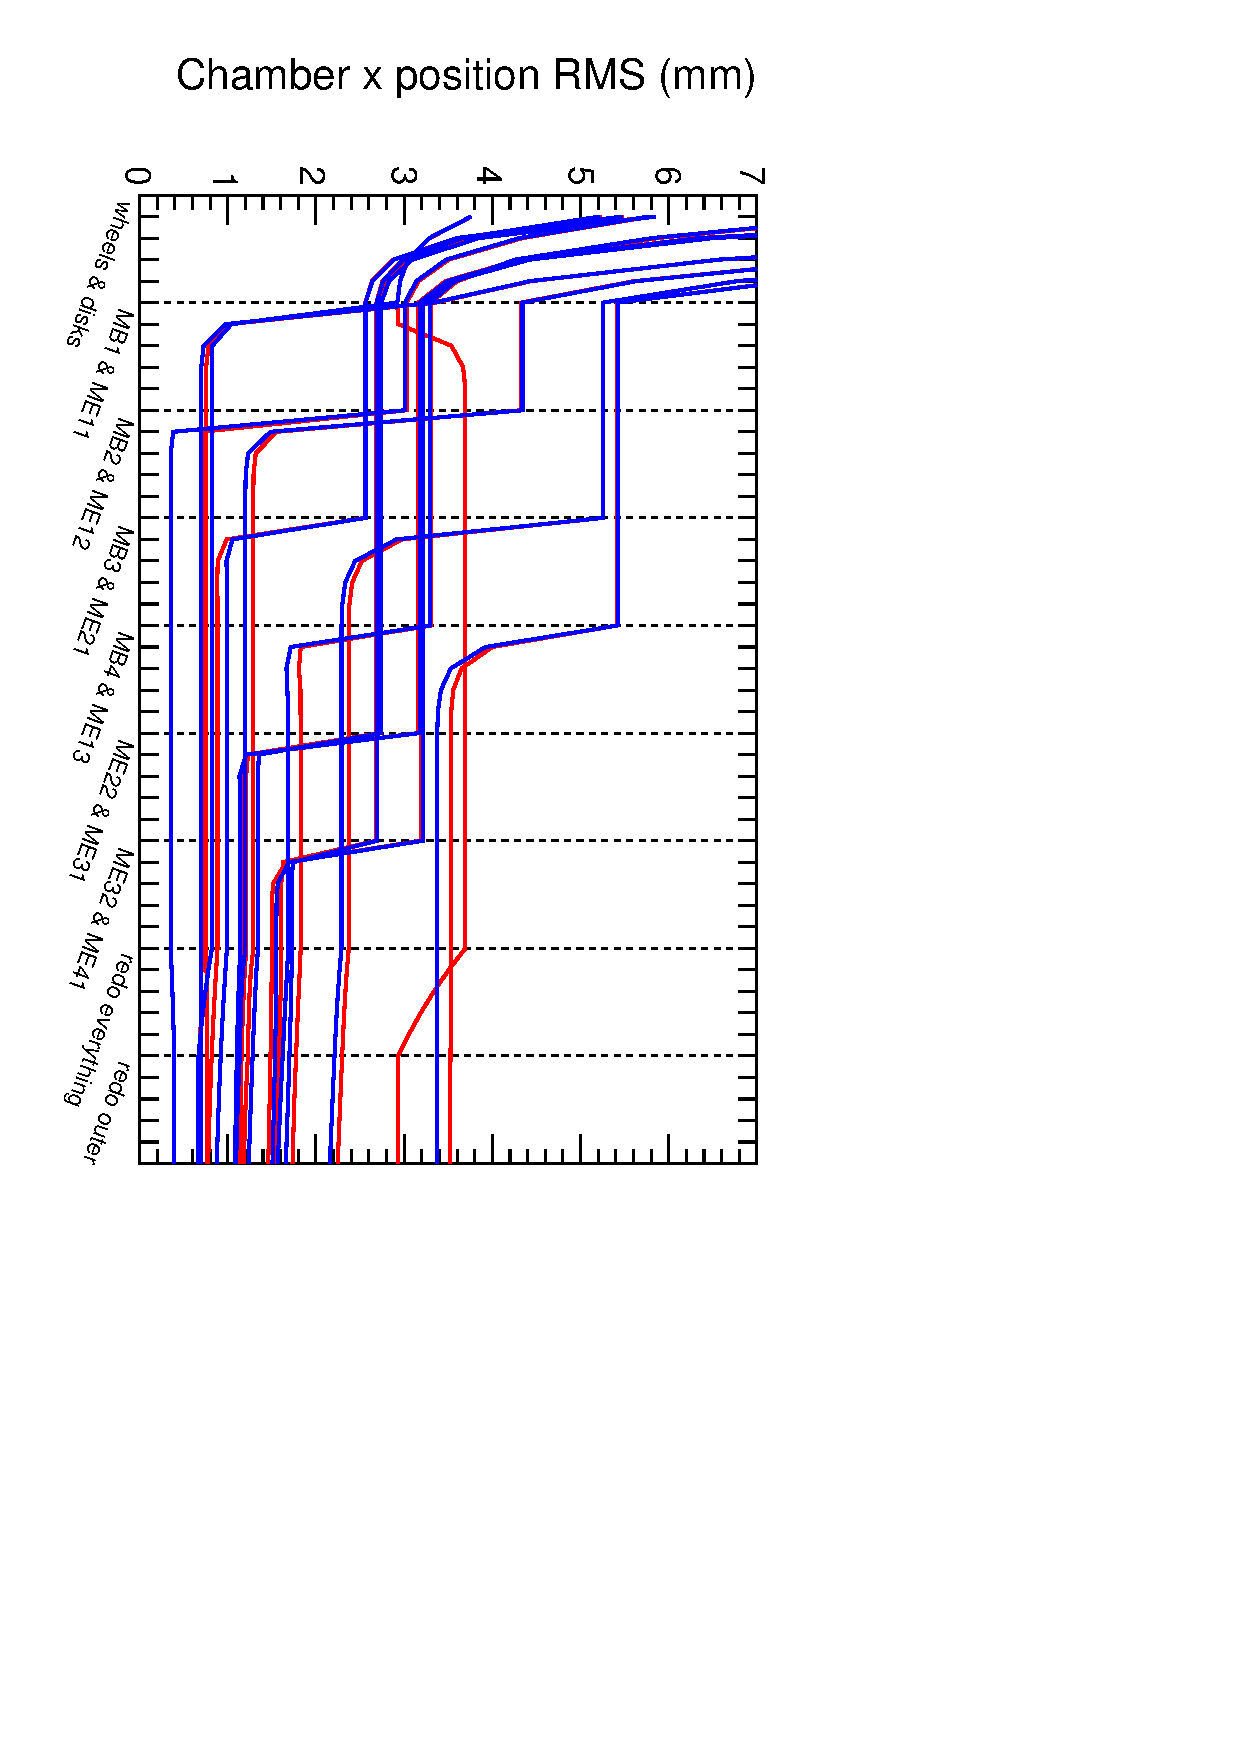
\includegraphics[height=0.95\linewidth, angle=90]{convergence_overlay.pdf}

\end{center}
\end{frame}

\begin{frame}
\frametitle{Why doesn't this error scale as $\sqrt{10}$?}
\begin{itemize}
\item Systematic error: means of residual distributions are well-measured, but don't correspond to chamber positions

\item {\it Example} scattering effect which can lead to bias:

\begin{center} 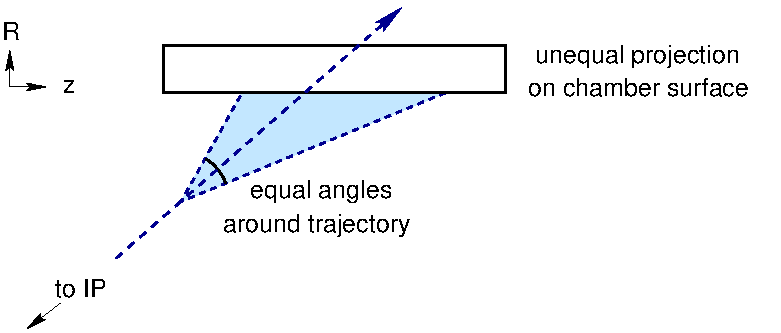
\includegraphics[width=7.5cm]{example.pdf} \end{center}

\item Errors compounded by fitting tracks to misaligned chambers

\item Tuning parameters (muon hit weight in fit) greatly reduces systematic
error in 100~pb$^{-1}$ alignment and increases statistical error; can
get close to $\sqrt{10}$ scaling

\end{itemize}
\end{frame}

\begin{frame}
\frametitle{What next?}
\begin{itemize}\setlength{\itemsep}{0.5 cm}
\item I optimize parameters for high-statistics procedure as a part of ongoing alignment work

\item Our testing method is valid, though it has been applied to a non-optimal alignment procedure

\item Text of the note makes it clear that we expect improvements to alignment procedures

\item Let's see the new plots (already commited to CVS)
\end{itemize}
\end{frame}

\begin{frame}
\frametitle{Dimuon spectra for lowest and highest mass}
Largely unchanged because alignment position errors are so similar

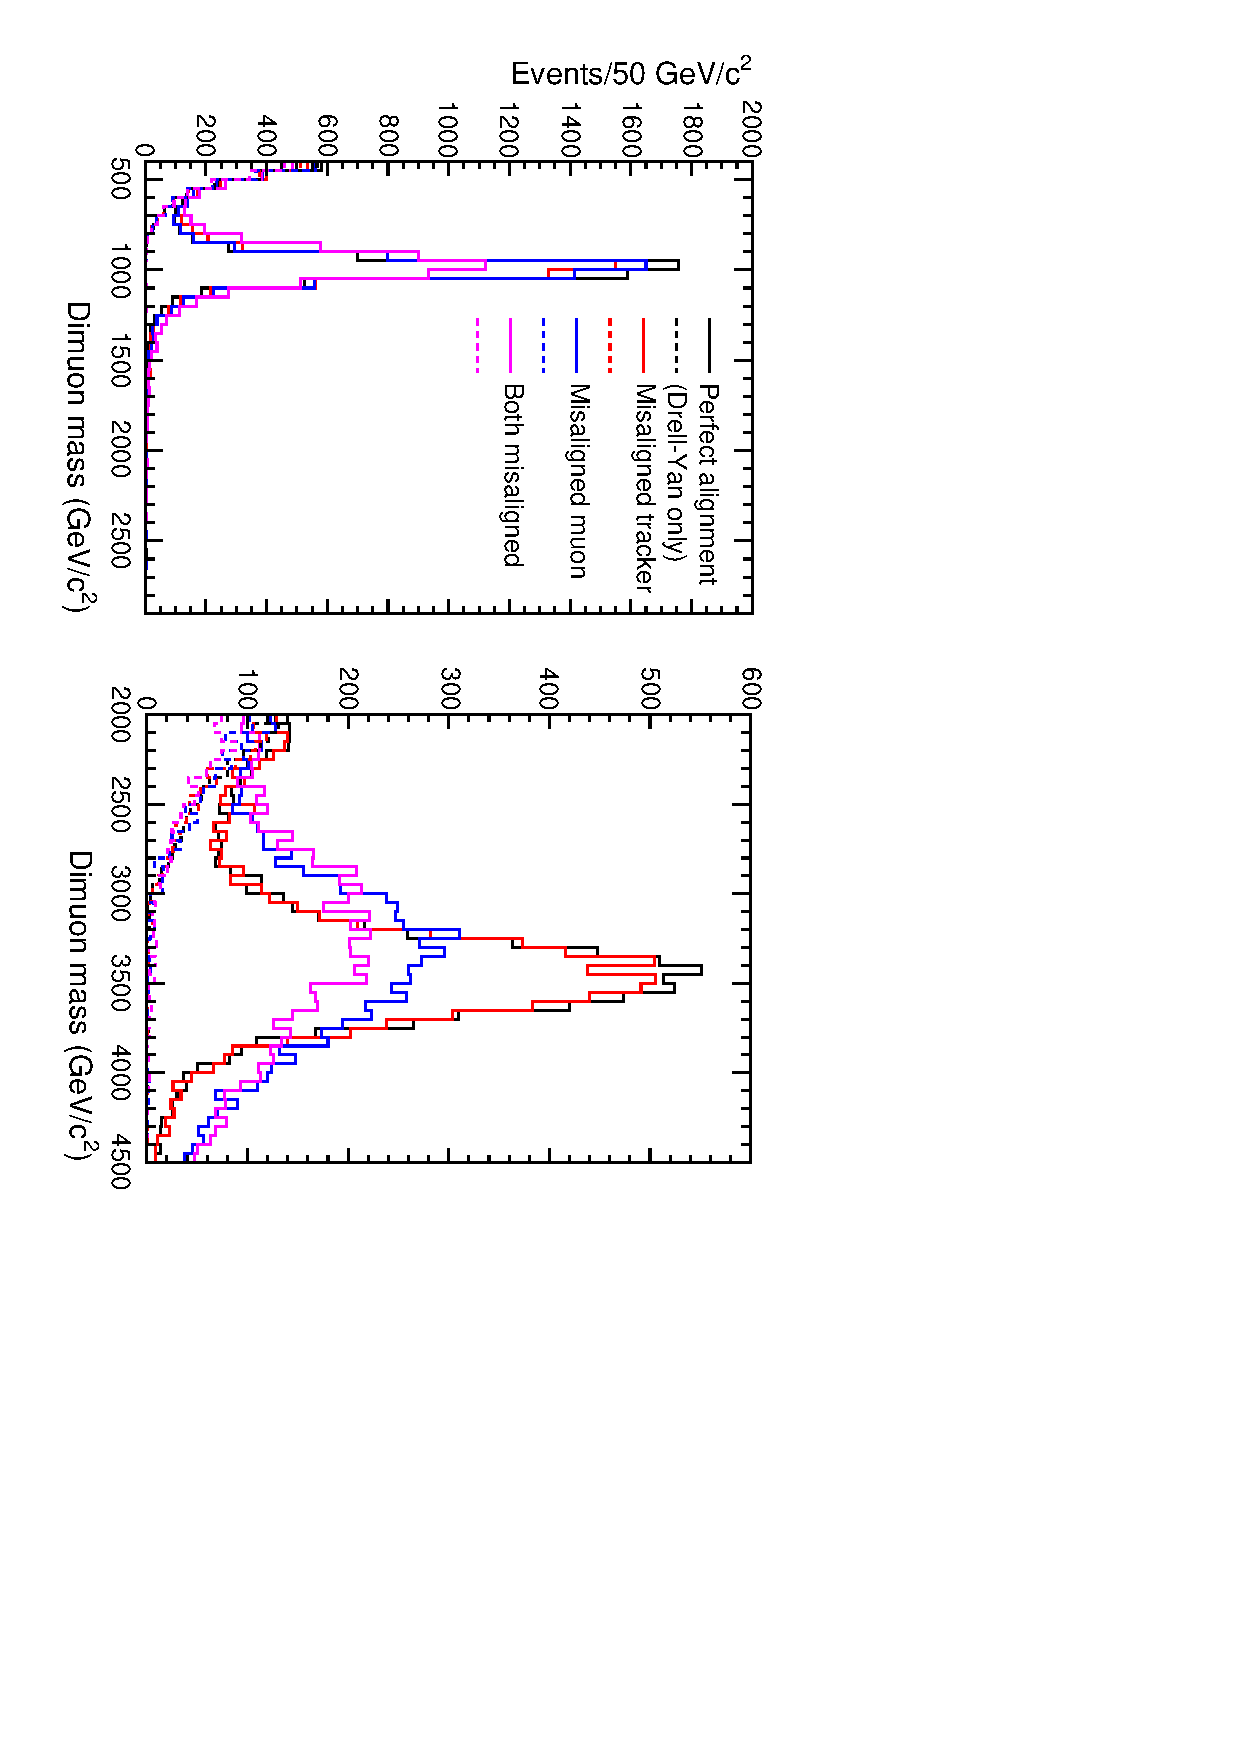
\includegraphics[height=\linewidth, angle=90]{ZSSM_Align100_Spectra_1000_3500.pdf}
\end{frame}

\begin{frame}
\frametitle{Resolution versus mass}
Largely unchanged because alignment position errors are so similar

\vspace{0.2 cm} New: tested procedure with three starting
configurations, gives us a sense of the uncertainty

\begin{center} 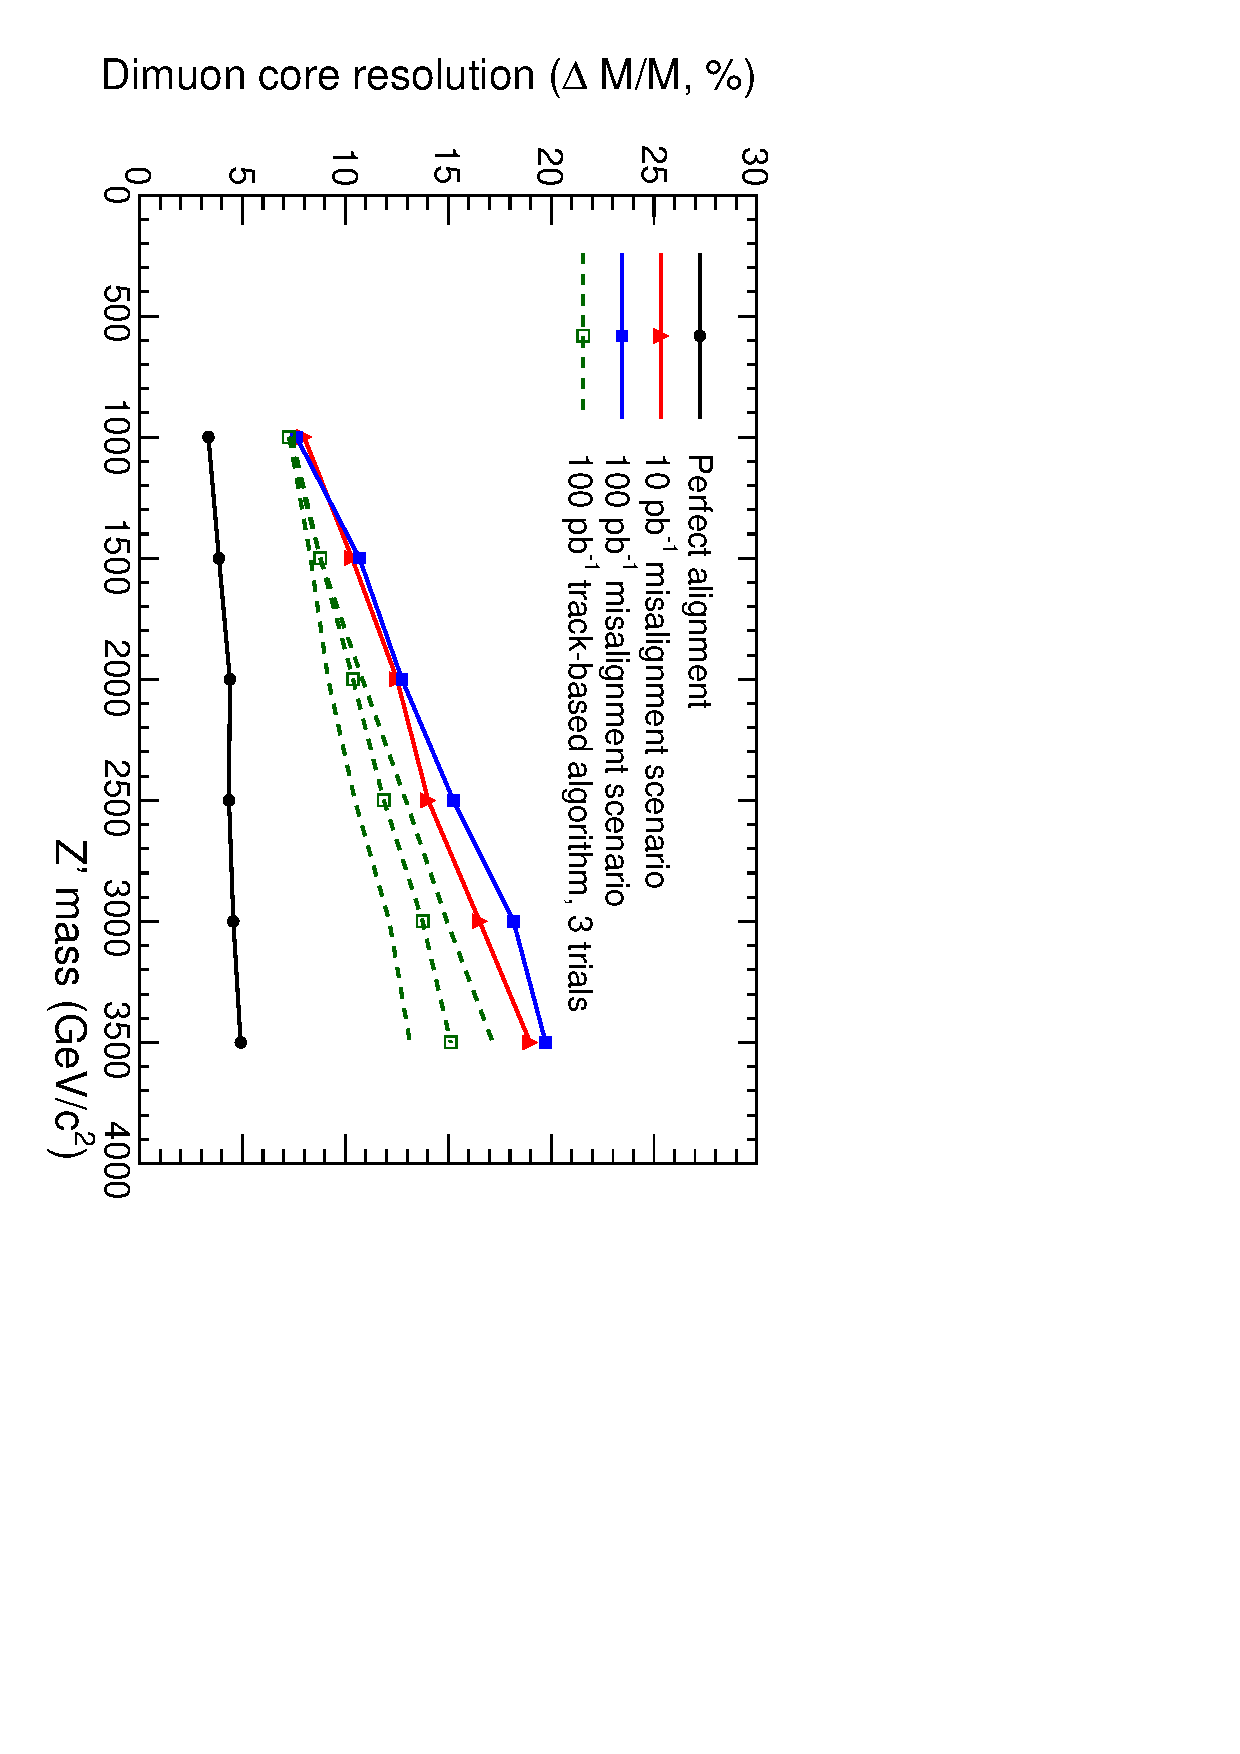
\includegraphics[height=0.8\linewidth, angle=90]{ZSSM_Align10-100_MassRes_color.pdf} \end{center}
\end{frame}

\begin{frame}
\frametitle{Raw resolution plots}
These are the fits that go into the plot on the previous page

\vspace{0.2 cm} 100~pb$^{-1}$ misalignment scenario (worst case)

\begin{center} 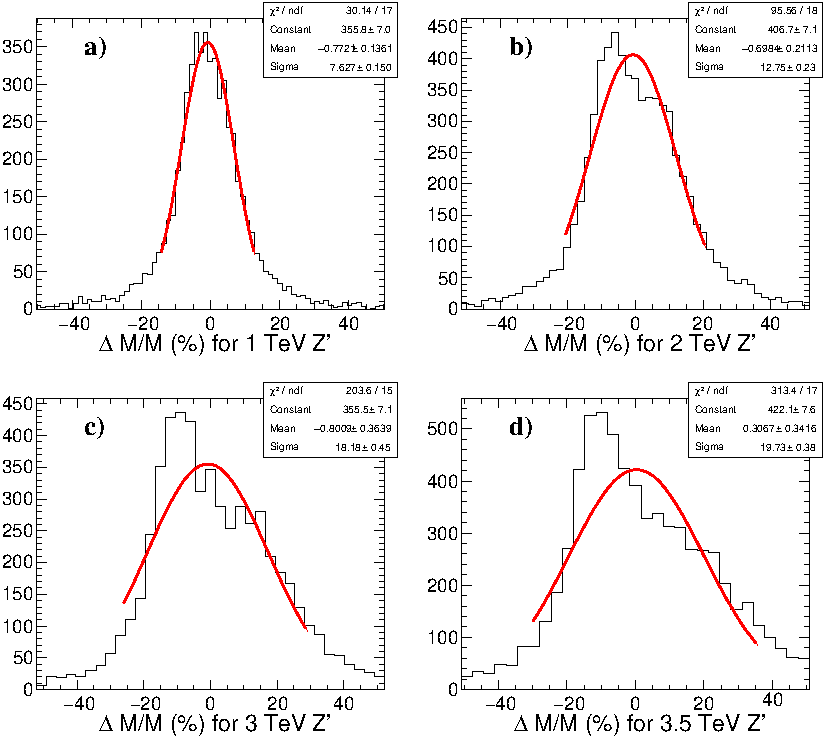
\includegraphics[width=0.6\linewidth]{four_plots.pdf} \end{center}
\end{frame}

%% \begin{frame}
%% \frametitle{Not in paper: resolution of individual tracks}
%% Largely unchanged because alignment position errors are so similar

%% 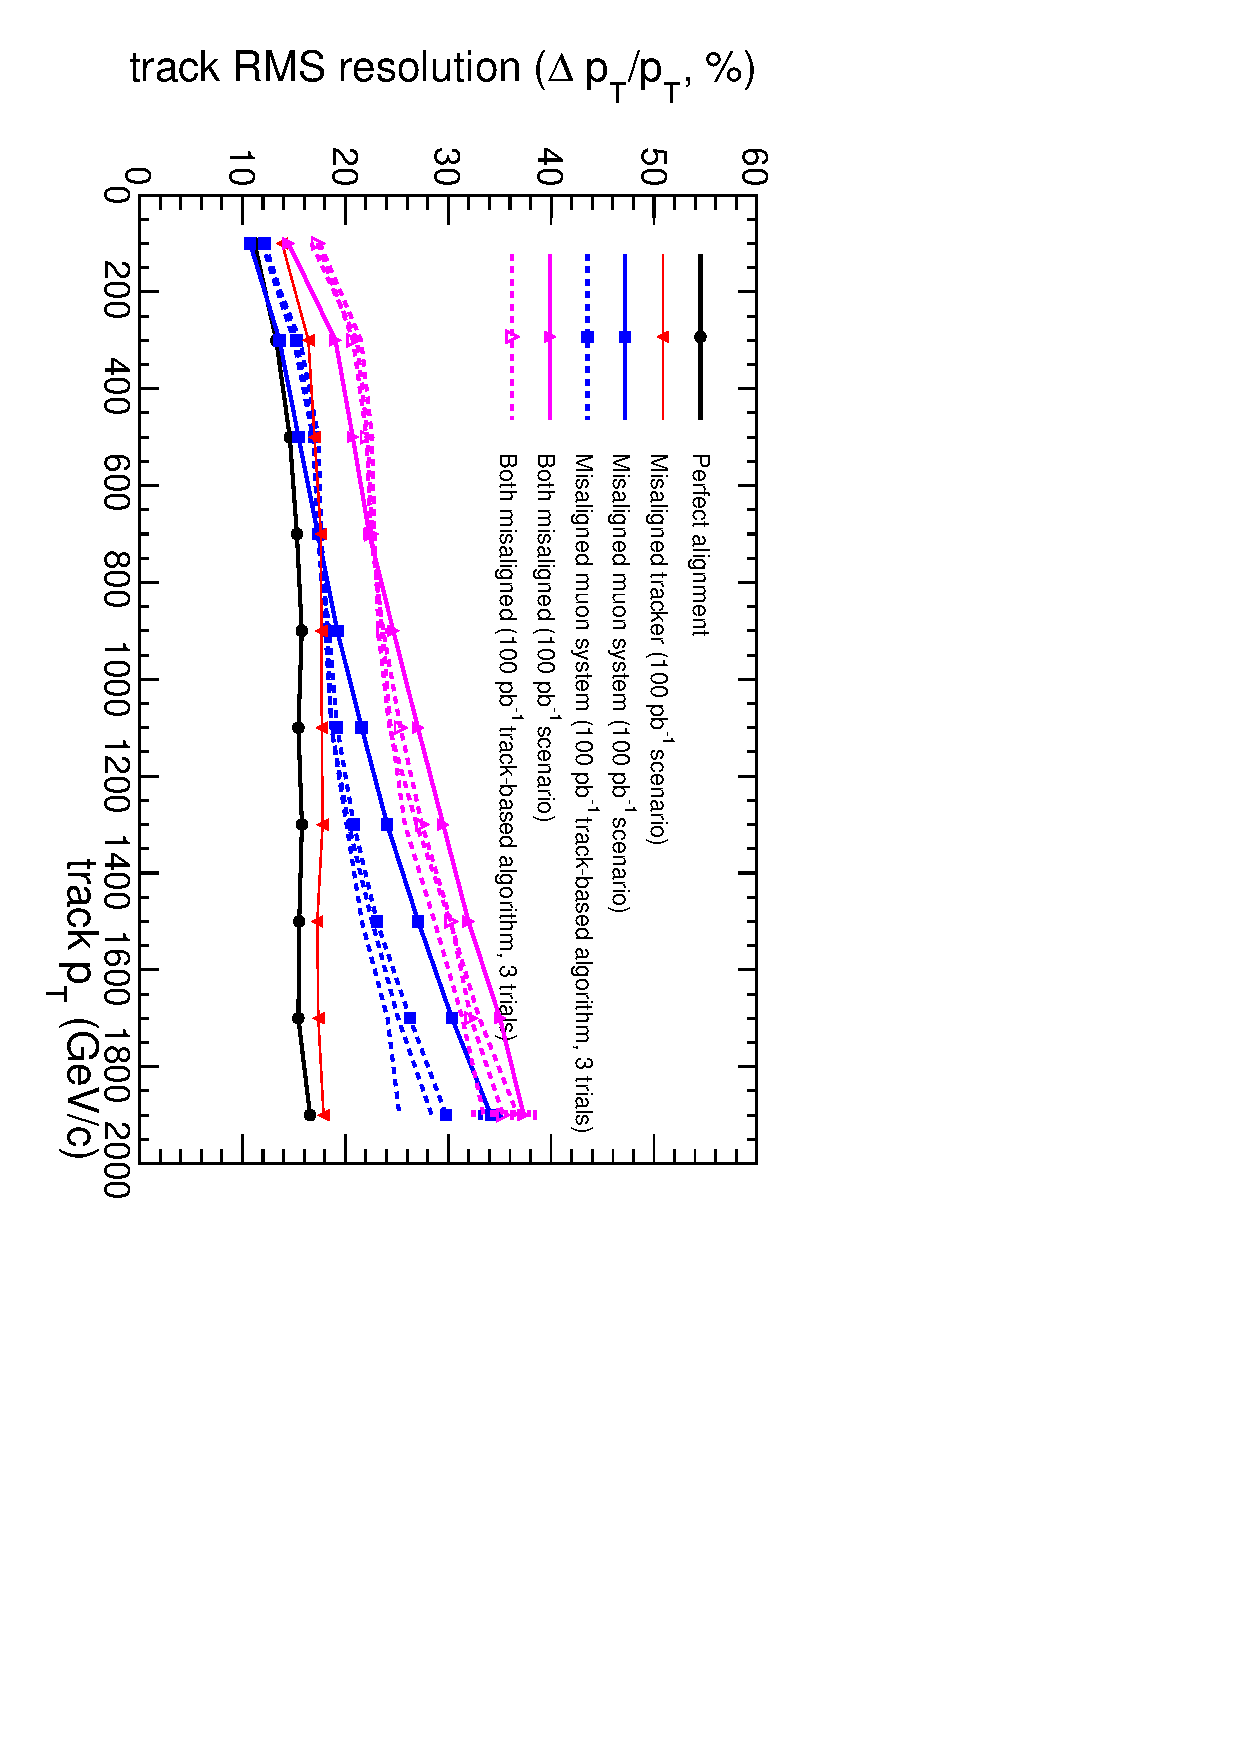
\includegraphics[height=\linewidth, angle=90]{ZSSM_Align_TrackRes_color-100.pdf}
%% \end{frame}

\begin{frame}
\frametitle{Bias can be seen on the level of tracks}
\begin{columns}
\column{0.5\linewidth}
\begin{center} Bias in track $p_T$ \end{center}

\vspace{-0.25 cm}
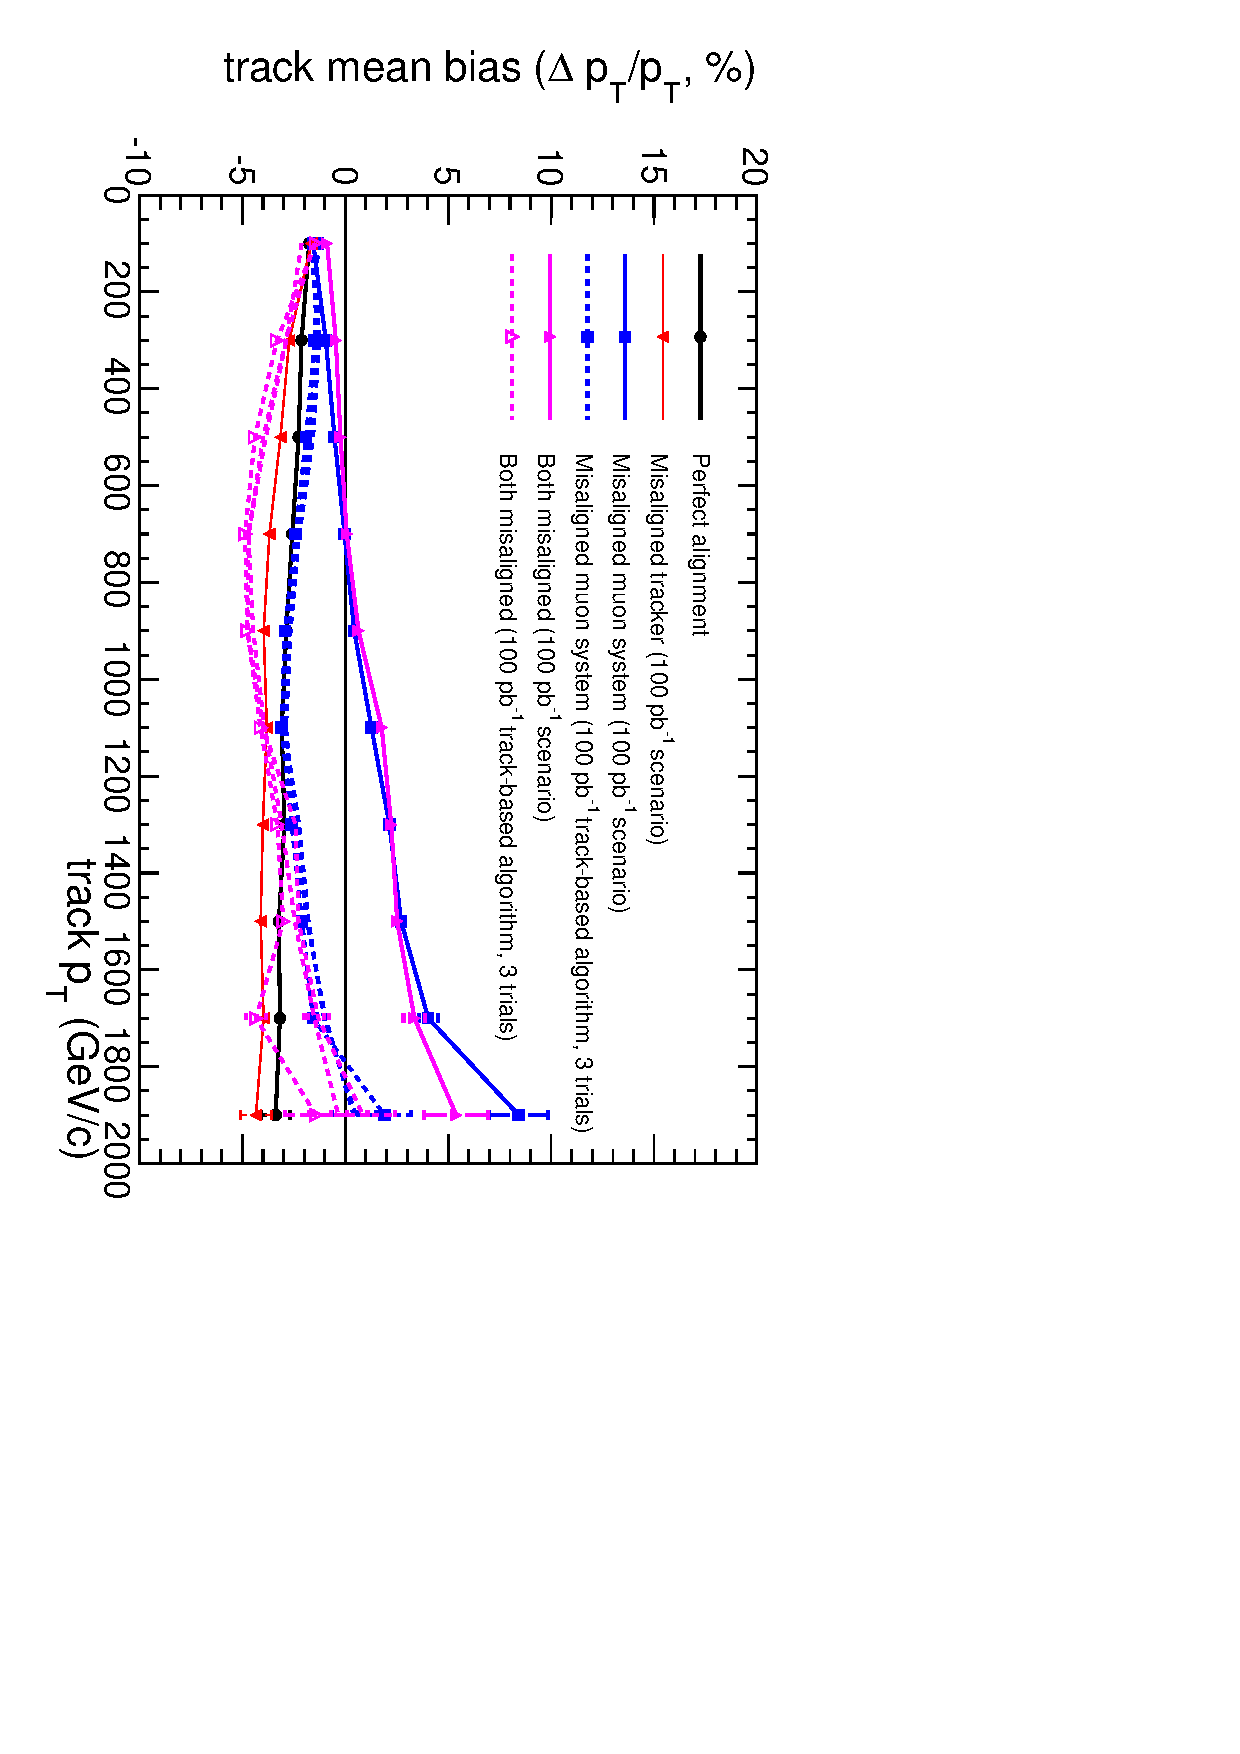
\includegraphics[height=\linewidth, angle=90]{ZSSM_Align_TrackBias_color-100.pdf}
\column{0.5\linewidth}
\begin{center} Bias in dimuon mass \end{center}

\vspace{-0.25 cm}
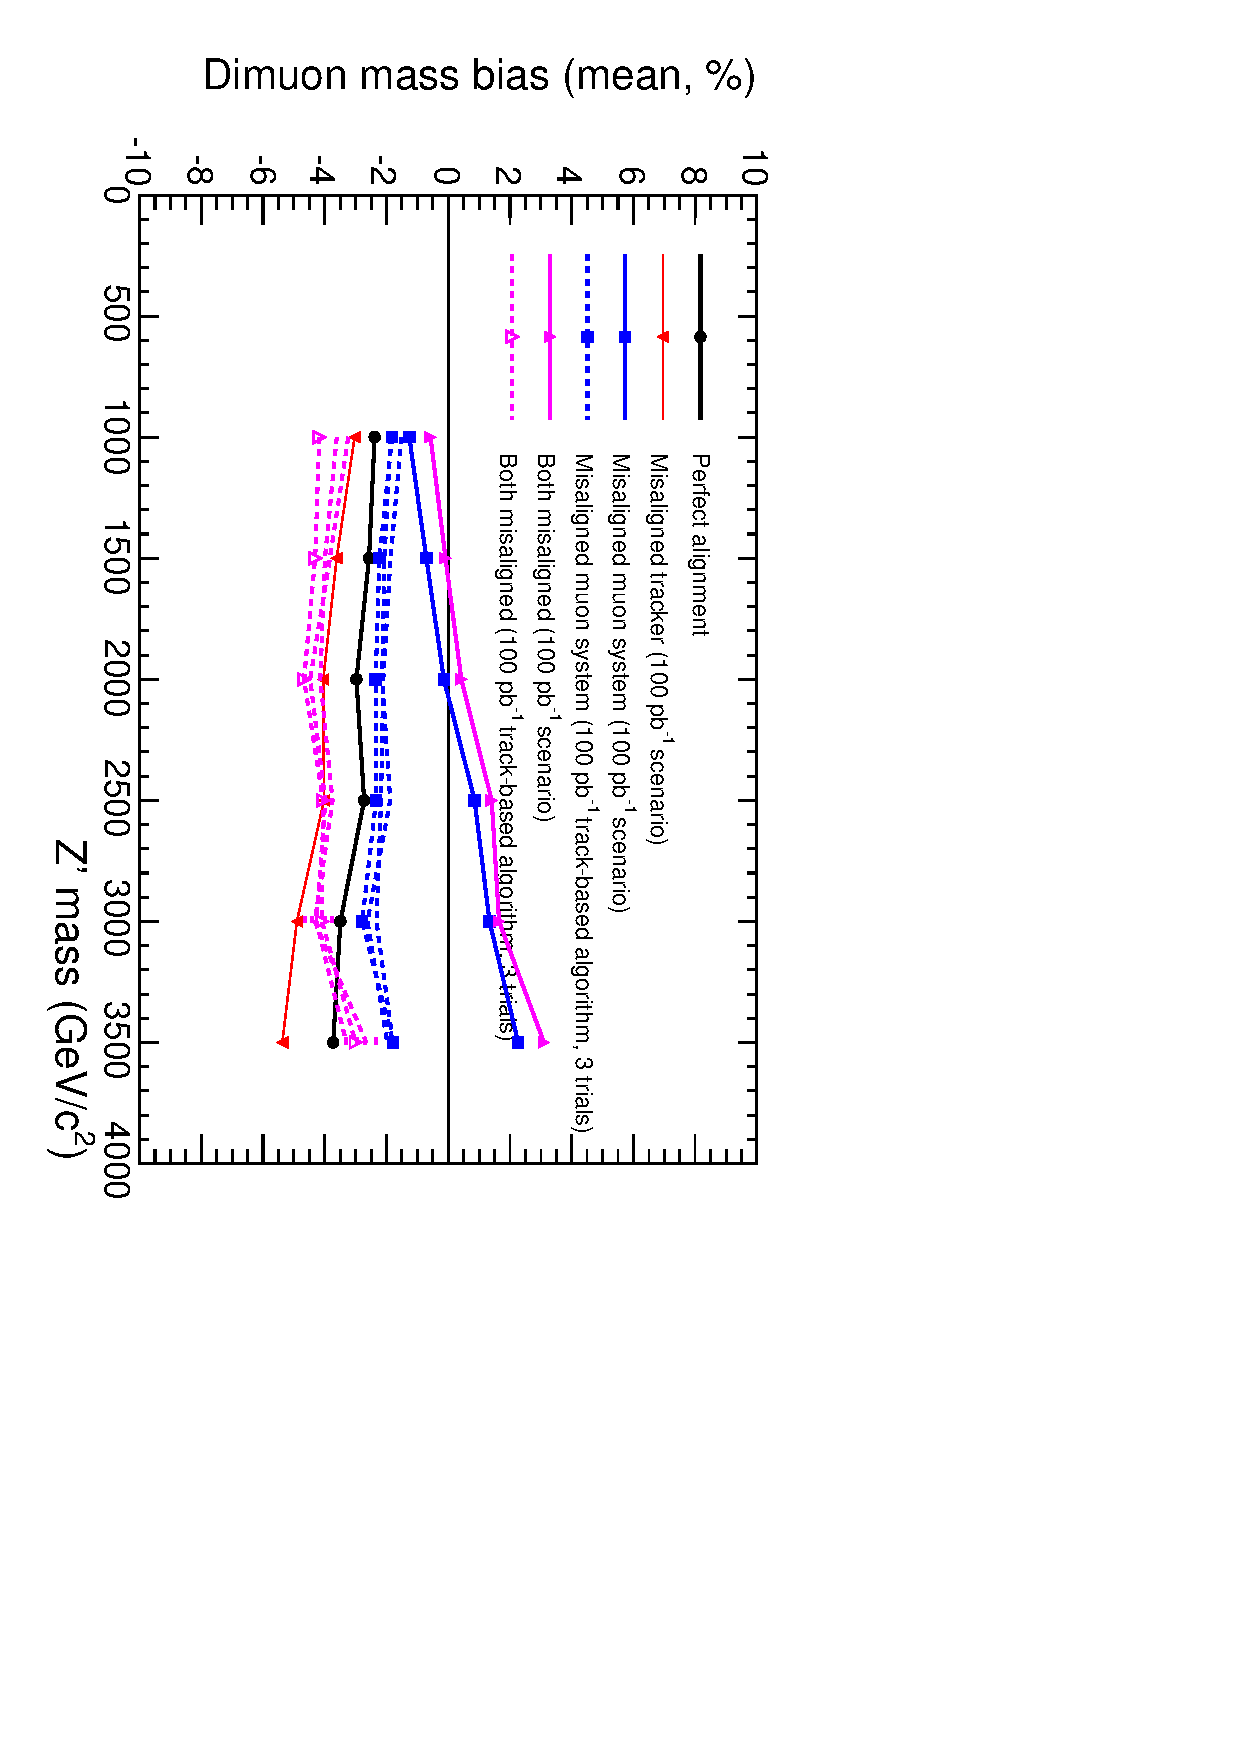
\includegraphics[height=\linewidth, angle=90]{ZSSM_Align_MassBiasMean_color-100.pdf}
\end{columns}

\vspace{0.5 cm} In both cases, we are looking at the mean of the

(reconstructed $-$ generated)$/$generated distribution

\vspace{0.5 cm} No more than 5\%
\end{frame}

\begin{frame}
\frametitle{Conclusions}
\begin{itemize}\setlength{\itemsep}{0.75 cm}
\item Measured effect of a non-optimal track-based alignment procedure
on TeV dimuons, verifying that the standard scenarios are in the right
ballpark (and may even be conservative)

\item Updated all the plots and the relevant text; answered all
FIXME's; everything has been committed to CVS

\item I'm still ready to answer questions and fill in more FIXME's
\end{itemize}

\label{numpages}
\end{frame}

\end{document}
